%%%%%%%%%%%%%%%%%%%%%%%%%%%%%%%%%%%%%%%%%%%%%%%%%%%%%%%%%%%%%%%%%%%%%%
% Supplementary Material (TMLR / OpenReview)
% HyperDG: Hyperbolic Representation Alignment for Robust Domain Generalization
%%%%%%%%%%%%%%%%%%%%%%%%%%%%%%%%%%%%%%%%%%%%%%%%%%%%%%%%%%%%%%%%%%%%%%

\documentclass[11pt]{article}

% ---------------- Packages ----------------
\usepackage[a4paper,margin=1in]{geometry}
\usepackage{amsmath,amssymb}
\usepackage{booktabs}
\usepackage{graphicx}
\usepackage{subcaption}
\usepackage{float}
\usepackage{multirow}
\usepackage{array}
\usepackage{hyperref}
\usepackage{xcolor}
\usepackage{enumitem}

\hypersetup{
colorlinks=true,
linkcolor=blue,
citecolor=blue,
urlcolor=blue
}

\title{\textbf{Supplementary Material}\\[4pt]
HyperDG: Does Per-Domain Hyperbolic Curvature Help Domain Generalization?\\
A Controlled Test on a Pretrained Backbone}

\author{Sunny Gupta \and Amit Sethi}

\date{}

\begin{document}
\maketitle
\vspace{-1em}

%%%%%%%%%%%%%%%%%%%%%%%%%%%%%%%%%%%%%%%%%%%%%%%%%%%%%%%%%%%%%%%%%%%%%%
\section{Overview}

This supplementary document accompanies the revised submission and contains additional visualizations, expanded ablations, and implementation details requested during review. In particular, we include:

\begin{itemize}[leftmargin=1.5em]
\item Per-dataset per-domain curvature trajectories with and without the
      variance regularizer ($\lambda_{\mathrm{var}}{=}0$ vs.\ $0.2$).
\item Class-prototype Poincar\'e disk visualizations across all
      datasets and conditions.
\item Single-shared-curvature vs.\ per-domain-curvature accuracy
      comparison (single-seed; corrected from earlier draft).
\item MERU backbone Poincar\'e visualizations.
\item Runtime cost and implementation notes.
\end{itemize}

\section{Per-dataset curvature trajectories}

Figures~\ref{fig:supp_traj_pacs}--\ref{fig:supp_traj_terra} show, per
dataset, the trajectory of each per-domain curvature parameter $K_i$
during training, under $\lambda_{\mathrm{var}}{=}0$ (left) and the default
$\lambda_{\mathrm{var}}{=}0.2$ (right). Each panel contains 4 leave-one-out
splits $\times$ 3 training domains $=$ 12 trajectories. The dashed
horizontal marks the initialization $K_{\mathrm{init}} \approx 0.6932$.
The key observation is that the left and right panels are visually almost
indistinguishable on every dataset: gradient dynamics alone are sufficient
to keep per-domain curvatures within a narrow band.

\begin{figure}[H]
\centering
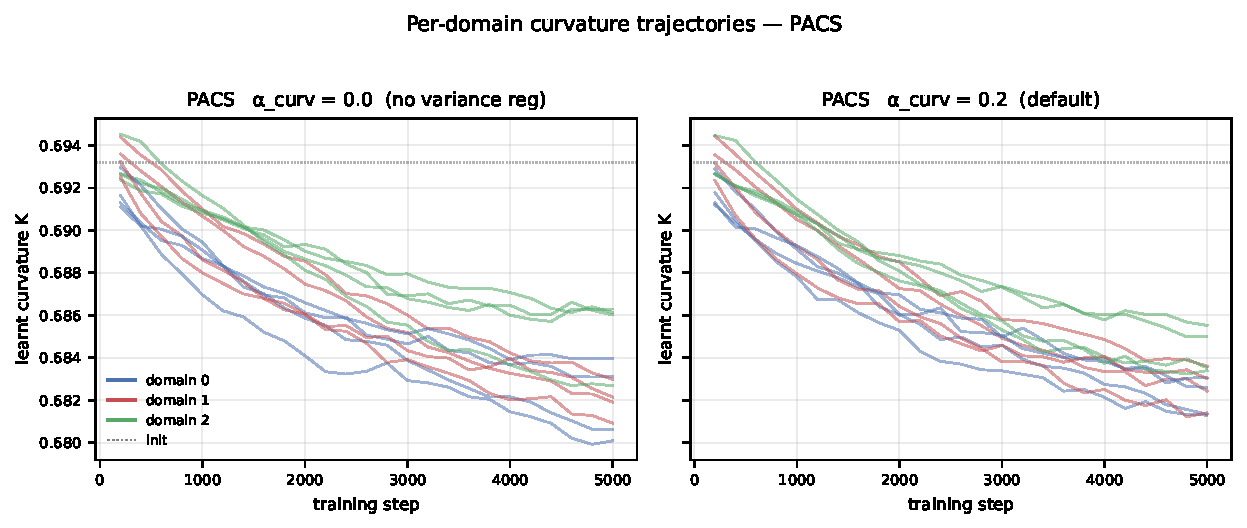
\includegraphics[width=0.88\linewidth]{fig_curvature_trajectories_pacs.pdf}
\caption{PACS curvature trajectories.}
\label{fig:supp_traj_pacs}
\end{figure}
\begin{figure}[H]
\centering
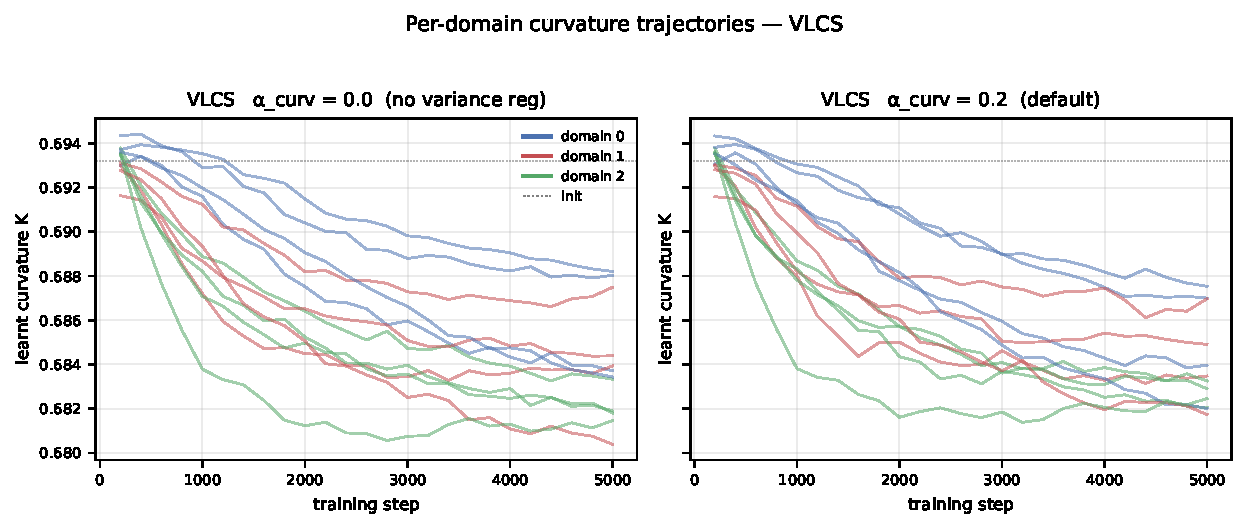
\includegraphics[width=0.88\linewidth]{fig_curvature_trajectories_vlcs.pdf}
\caption{VLCS curvature trajectories.}
\label{fig:supp_traj_vlcs}
\end{figure}
\begin{figure}[H]
\centering
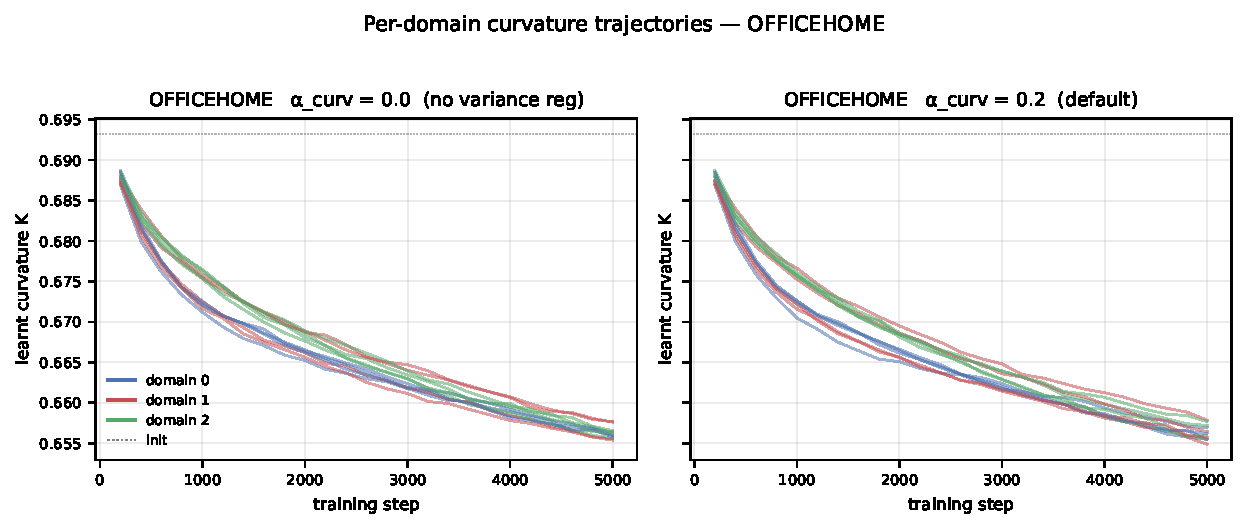
\includegraphics[width=0.88\linewidth]{fig_curvature_trajectories_officehome.pdf}
\caption{OfficeHome curvature trajectories.}
\label{fig:supp_traj_oh}
\end{figure}
\begin{figure}[H]
\centering
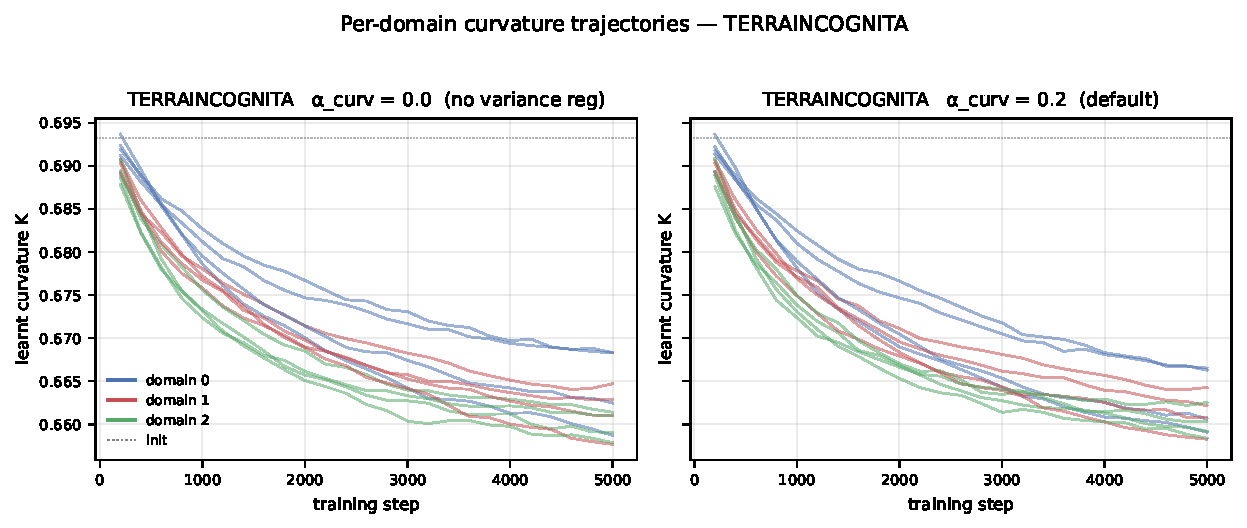
\includegraphics[width=0.88\linewidth]{fig_curvature_trajectories_terra.pdf}
\caption{TerraIncognita curvature trajectories.}
\label{fig:supp_traj_terra}
\end{figure}

%%%%%%%%%%%%%%%%%%%%%%%%%%%%%%%%%%%%%%%%%%%%%%%%%%%%%%%%%%%%%%%%%%%%%%
\section{Poincar\'e Disk Visualizations}

We project learned Lorentz embeddings into the Poincar\'e disk using:

\begin{enumerate}[leftmargin=1.5em]
\item Tangent-space extraction,
\item PCA reduction to 2D,
\item Exponential map with fixed curvature $K=-1$,
\item Stereographic projection.
\end{enumerate}

These figures qualitatively illustrate the geometric structure learned by HyperDG.

%%%%%%%%%%%%%%%%%%%%%%%%%%%%%%%%%%%%%%%%%%%%%%%%%%%%%%%%%%%%%%%%%%%%%%
\subsection{HyperDG (Per-Domain Curvature)}

\begin{figure}[H]
\centering

\begin{subfigure}{0.48\textwidth}
\centering
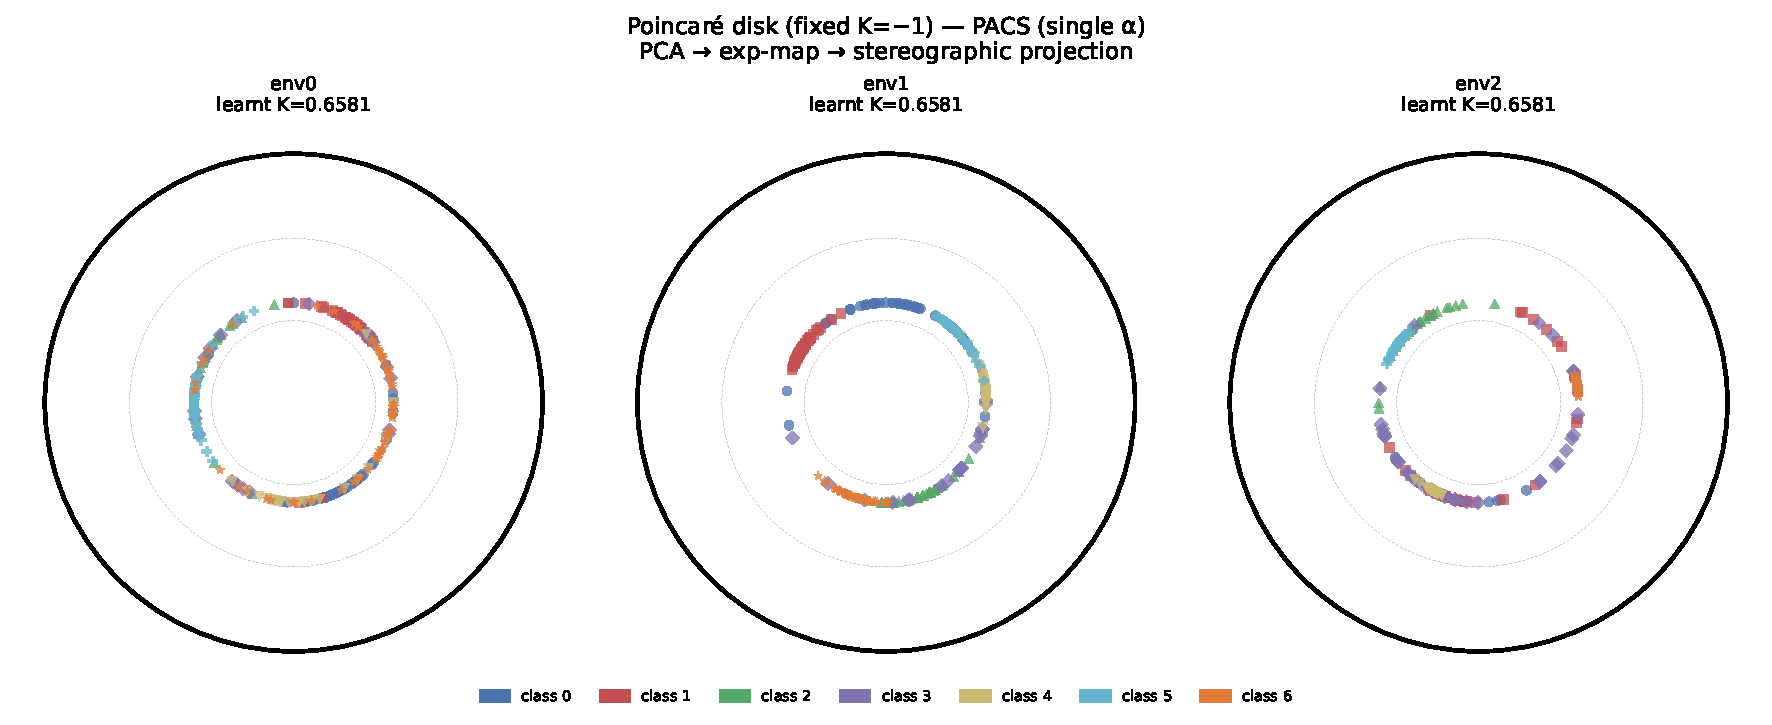
\includegraphics[width=\linewidth]{poincare_hyperdg_pacs_perdomain.pdf}
\caption{PACS}
\end{subfigure}
\hfill
\begin{subfigure}{0.48\textwidth}
\centering
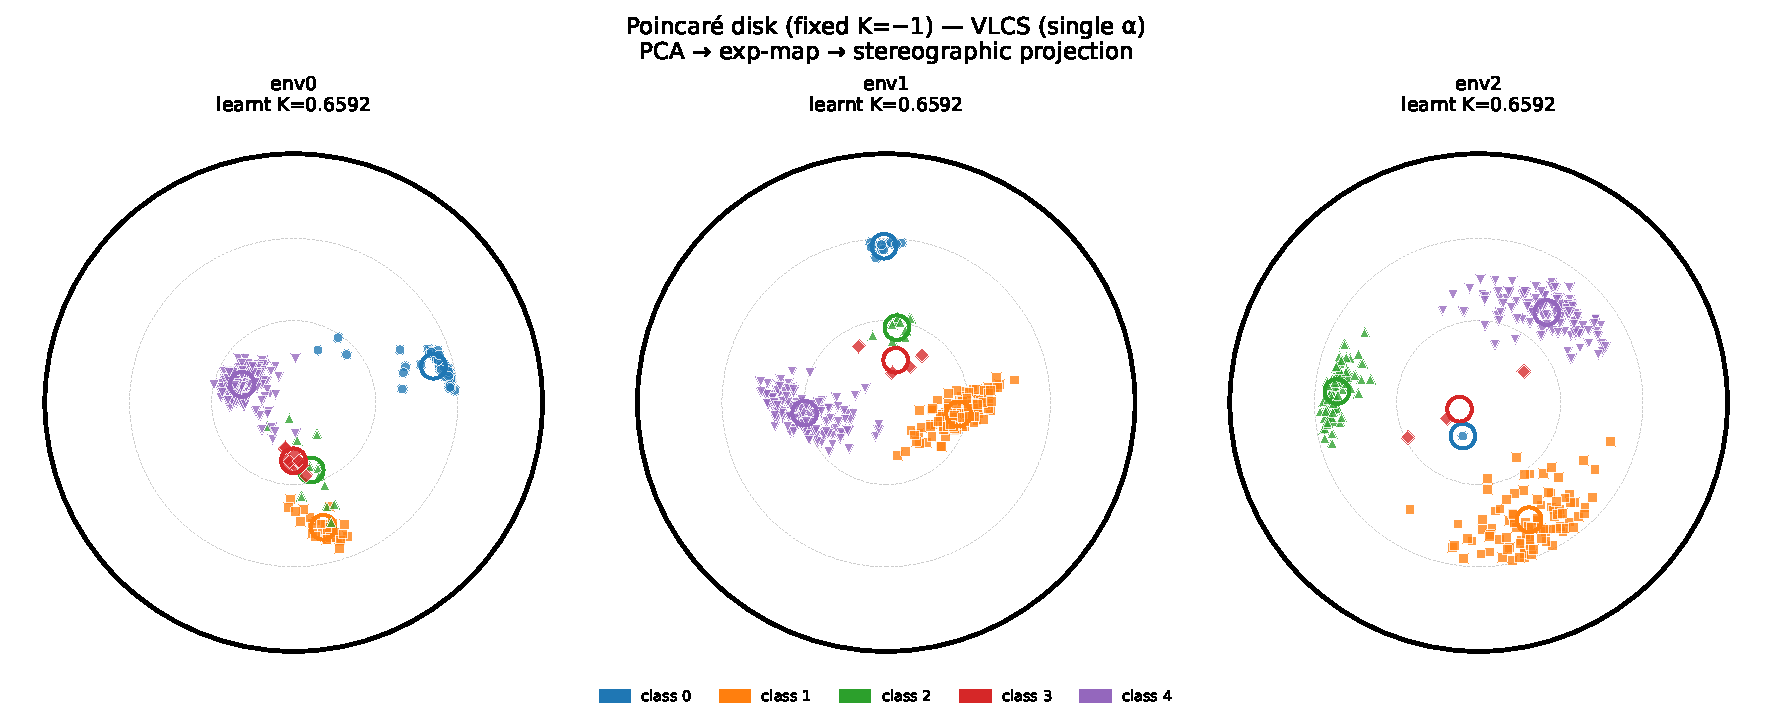
\includegraphics[width=\linewidth]{poincare_hyperdg_vlcs_perdomain.pdf}
\caption{VLCS}
\end{subfigure}

\vspace{0.5em}

\begin{subfigure}{0.48\textwidth}
\centering
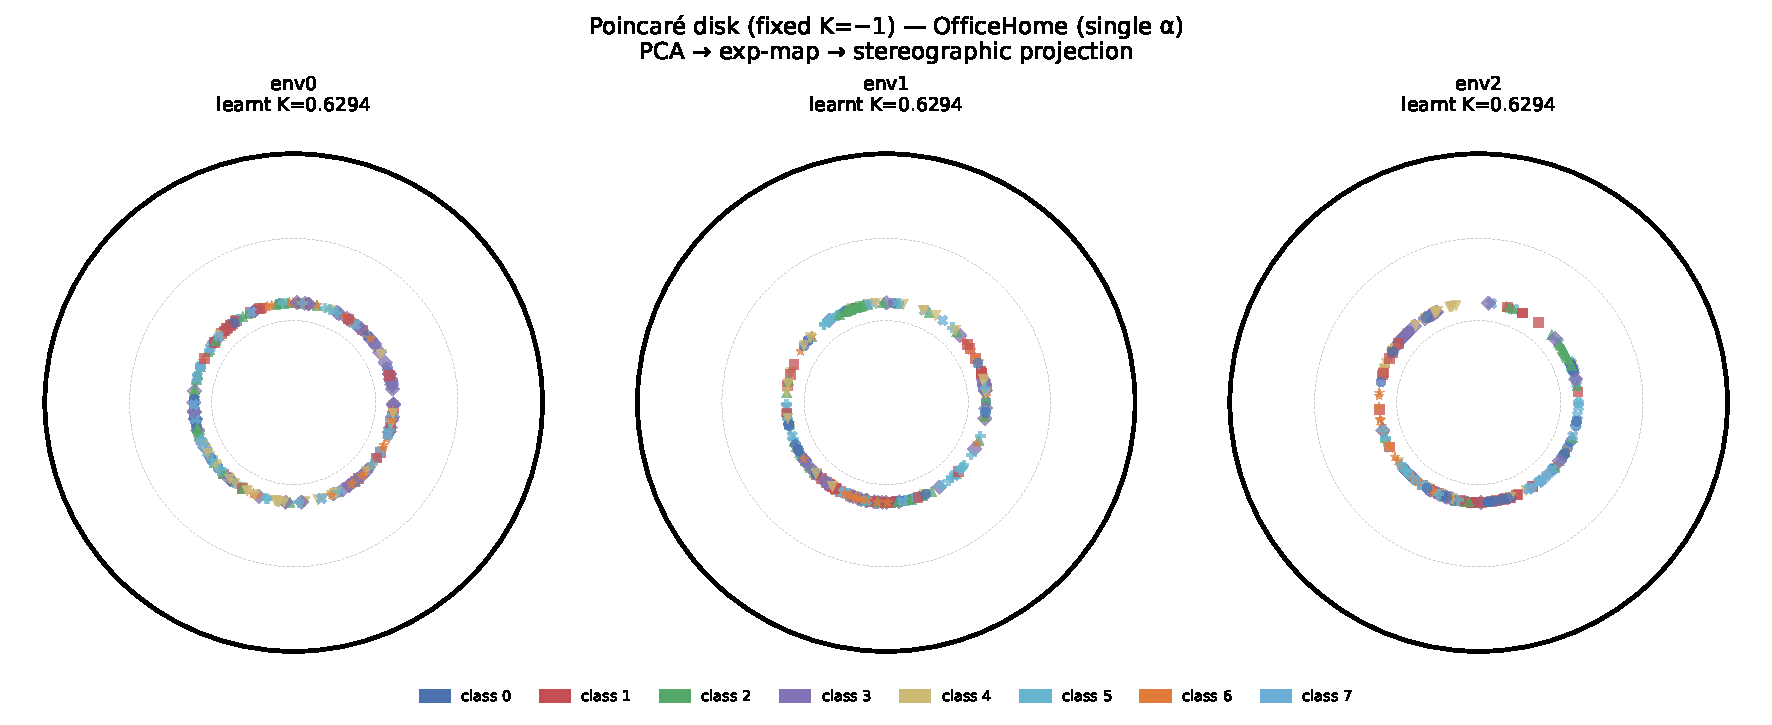
\includegraphics[width=\linewidth]{poincare_hyperdg_officehome_perdomain.pdf}
\caption{OfficeHome}
\end{subfigure}
\hfill
\begin{subfigure}{0.48\textwidth}
\centering
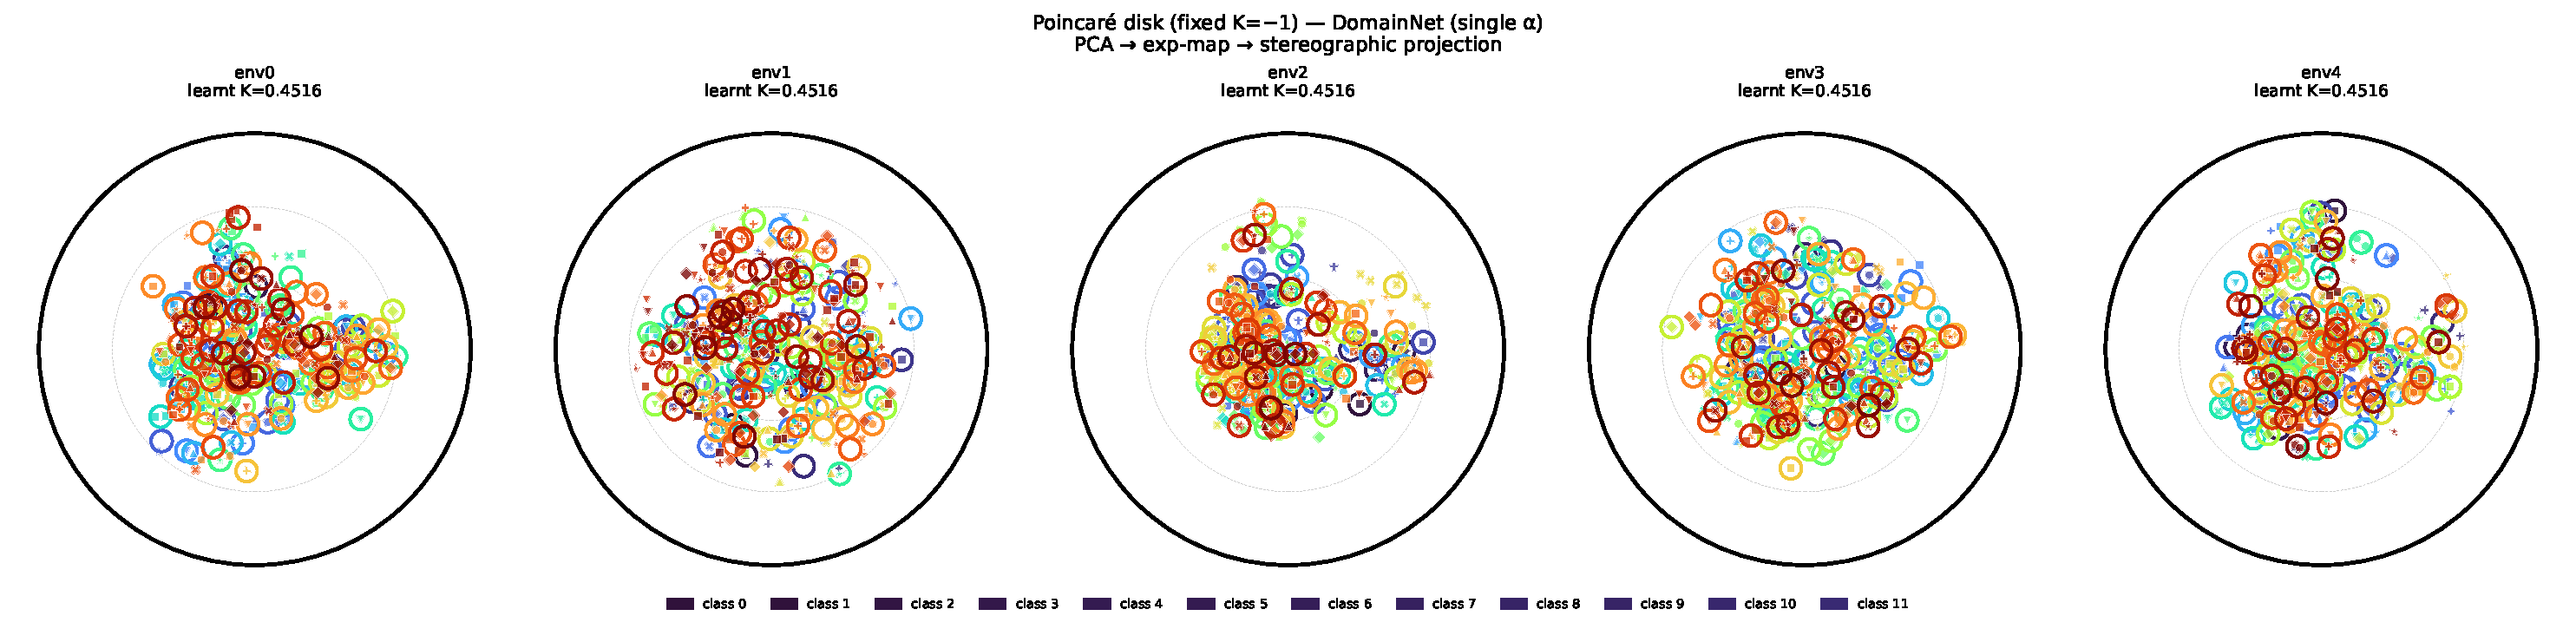
\includegraphics[width=\linewidth]{poincare_hyperdg_domainnet_perdomain.pdf}
\caption{DomainNet}
\end{subfigure}
\begin{subfigure}{0.48\textwidth}
\centering
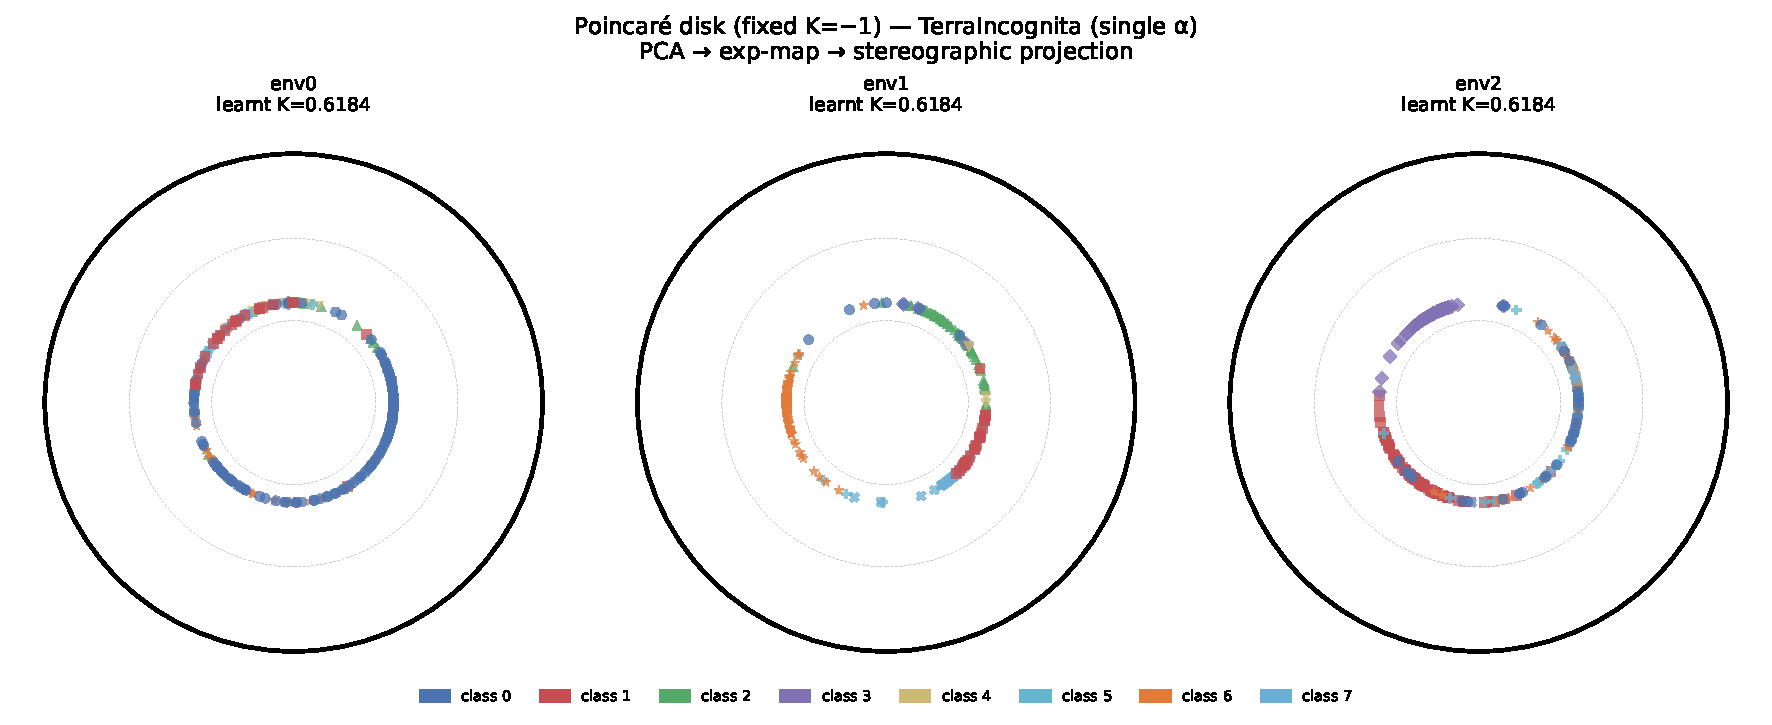
\includegraphics[width=\linewidth]{poincare_hyperdg_terra_perdomain.pdf}
\caption{DomainNet}
\end{subfigure}

\caption{HyperDG using per-domain learnable curvatures. Distinct radial cluster depths indicate geometry specialization across domains.}
\end{figure}

%%%%%%%%%%%%%%%%%%%%%%%%%%%%%%%%%%%%%%%%%%%%%%%%%%%%%%%%%%%%%%%%%%%%%%
%%%%%%%%%%%%%%%%%%%%%%%%%%%%%%%%%%%%%%%%%%%%%%%%%%%%%%%%%%%%%%%%%%%%%%
\subsection{HyperDG (Single Shared Curvature)}

\begin{figure}[H]
\centering

\begin{subfigure}{0.48\textwidth}
\centering
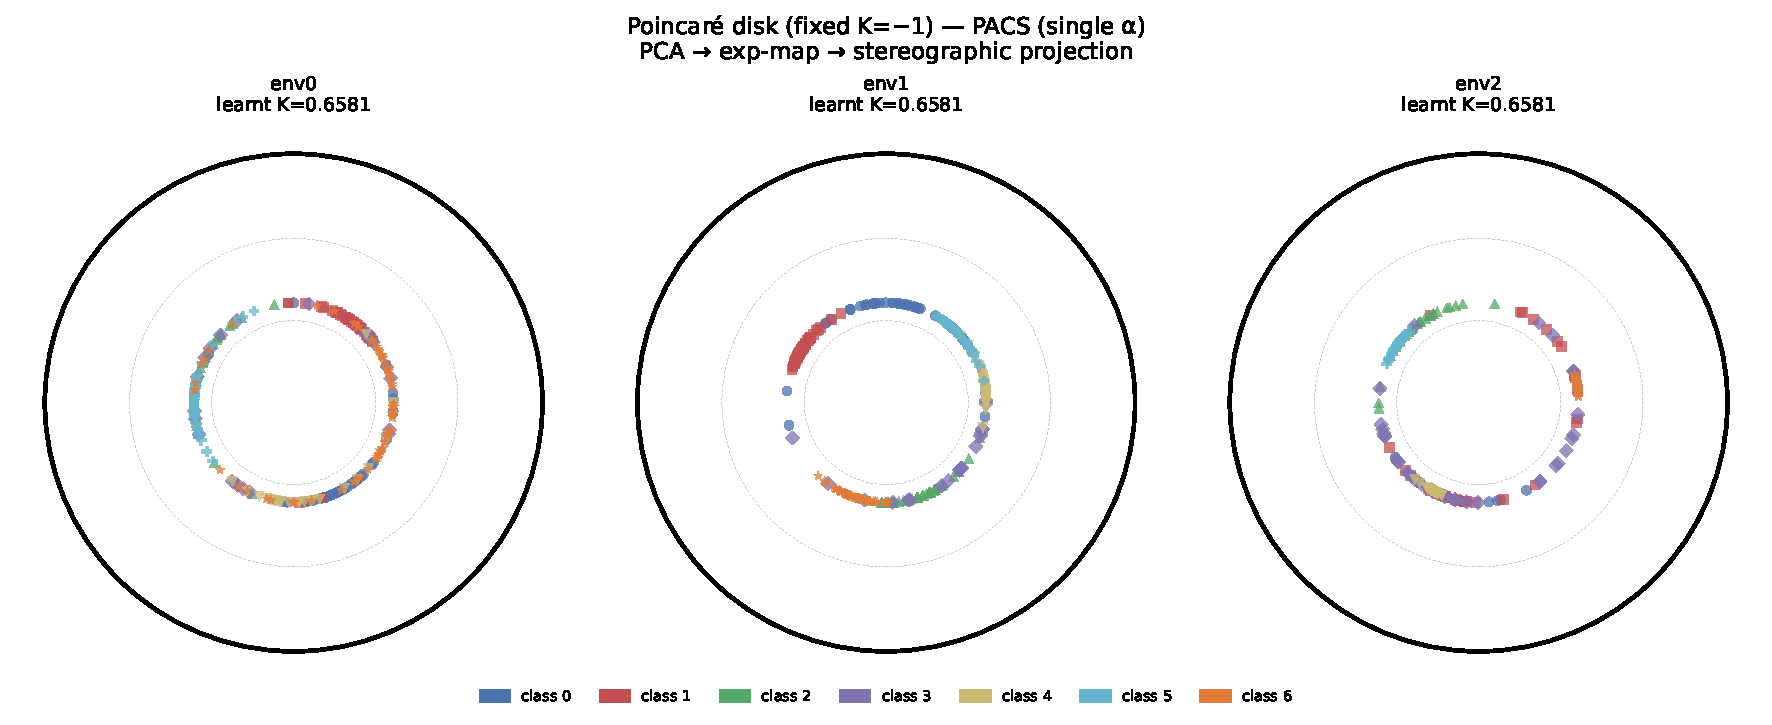
\includegraphics[width=\linewidth]{poincare_hyperdg_pacs_singlecurv.pdf}
\caption{PACS}
\end{subfigure}
\hfill
\begin{subfigure}{0.48\textwidth}
\centering
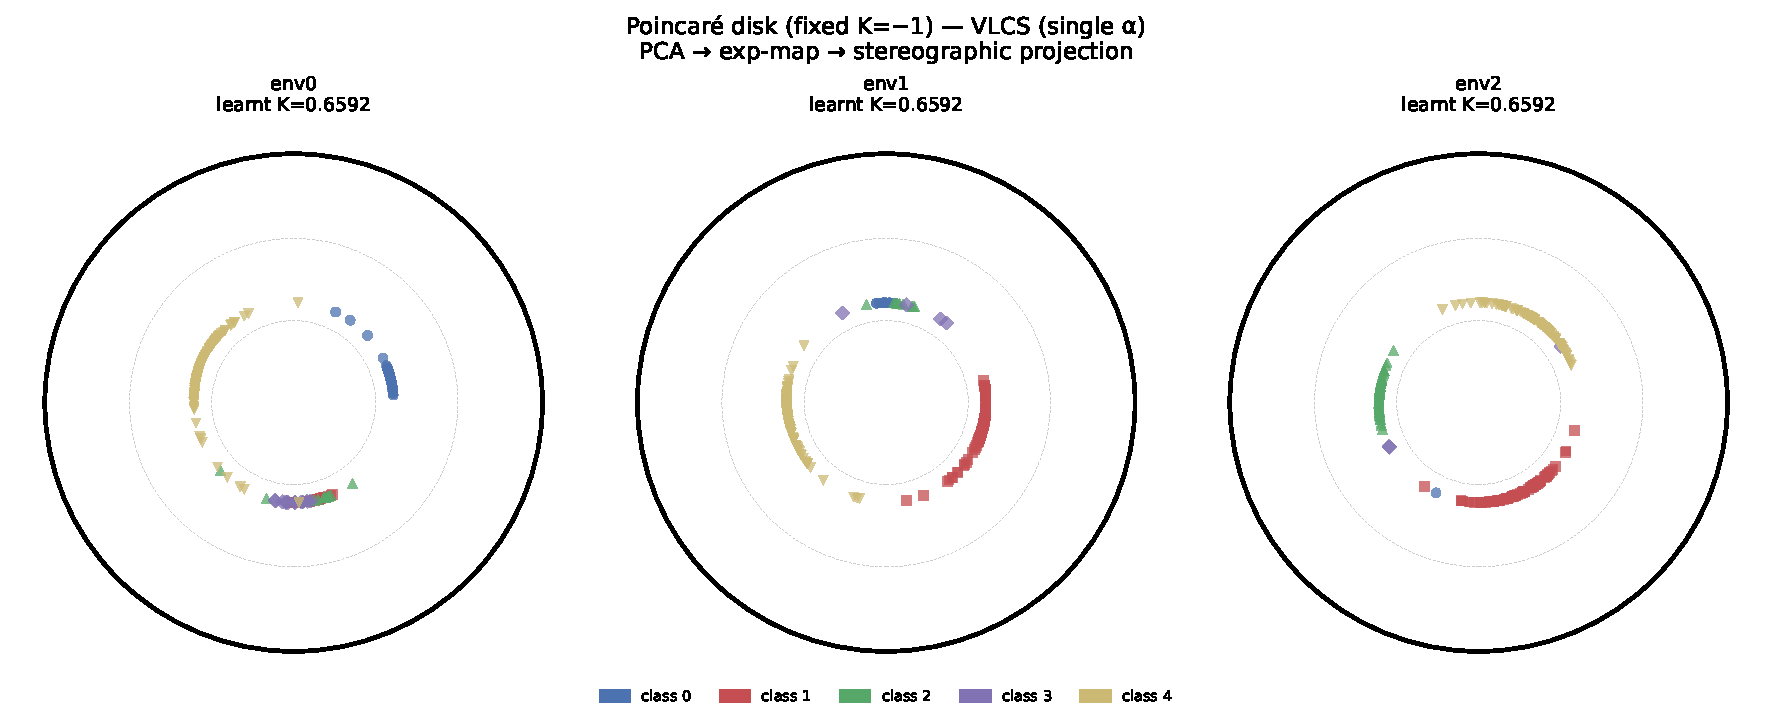
\includegraphics[width=\linewidth]{poincare_hyperdg_vlcs_singlecurv.pdf}
\caption{VLCS}
\end{subfigure}

\vspace{0.5em}

\begin{subfigure}{0.48\textwidth}
\centering
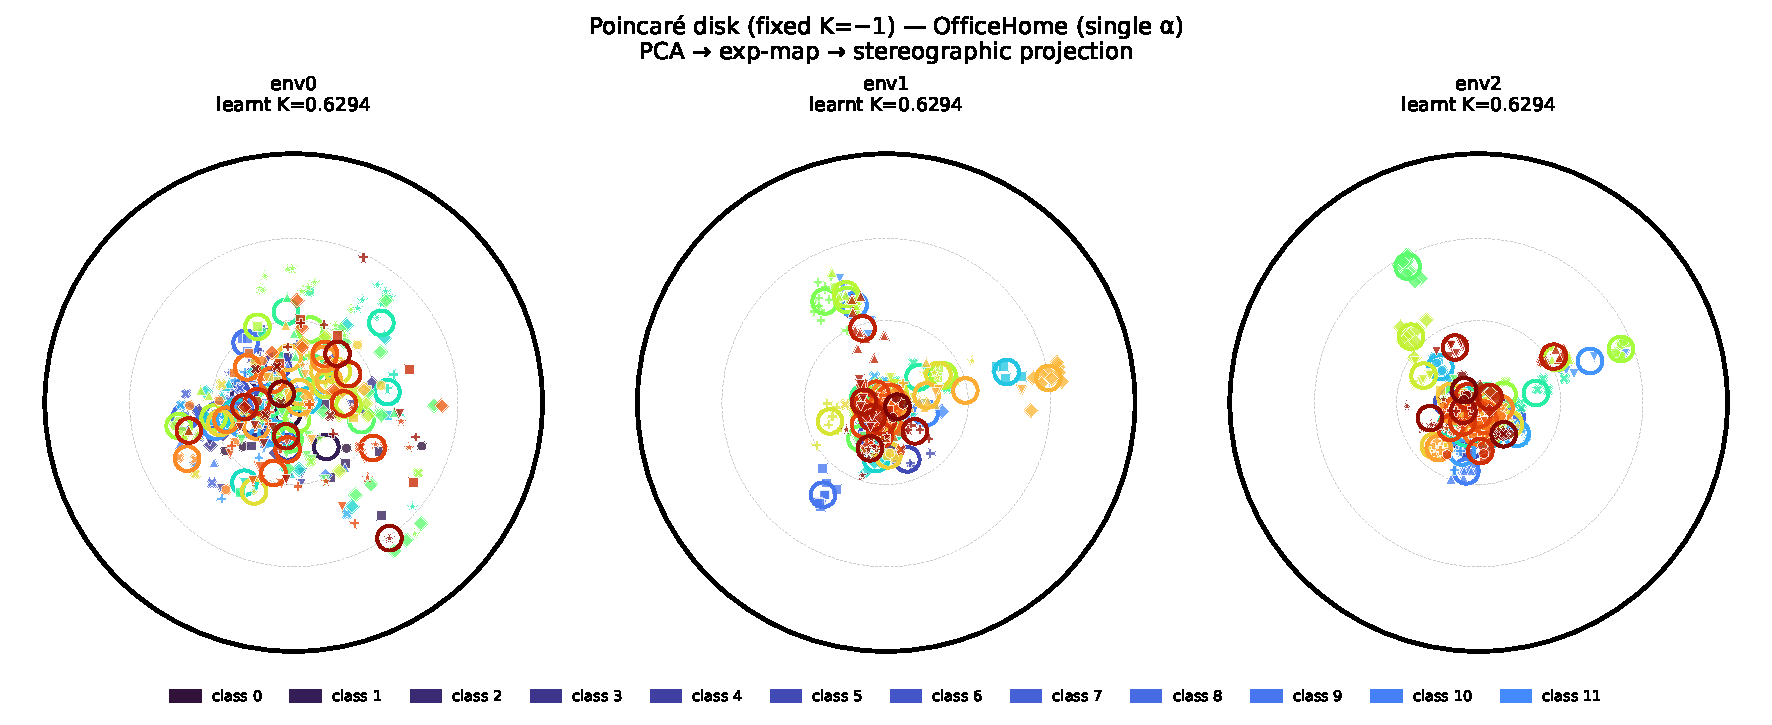
\includegraphics[width=\linewidth]{poincare_hyperdg_officehome_singlecurv.pdf}
\caption{OfficeHome}
\end{subfigure}
\hfill
\begin{subfigure}{0.48\textwidth}
\centering
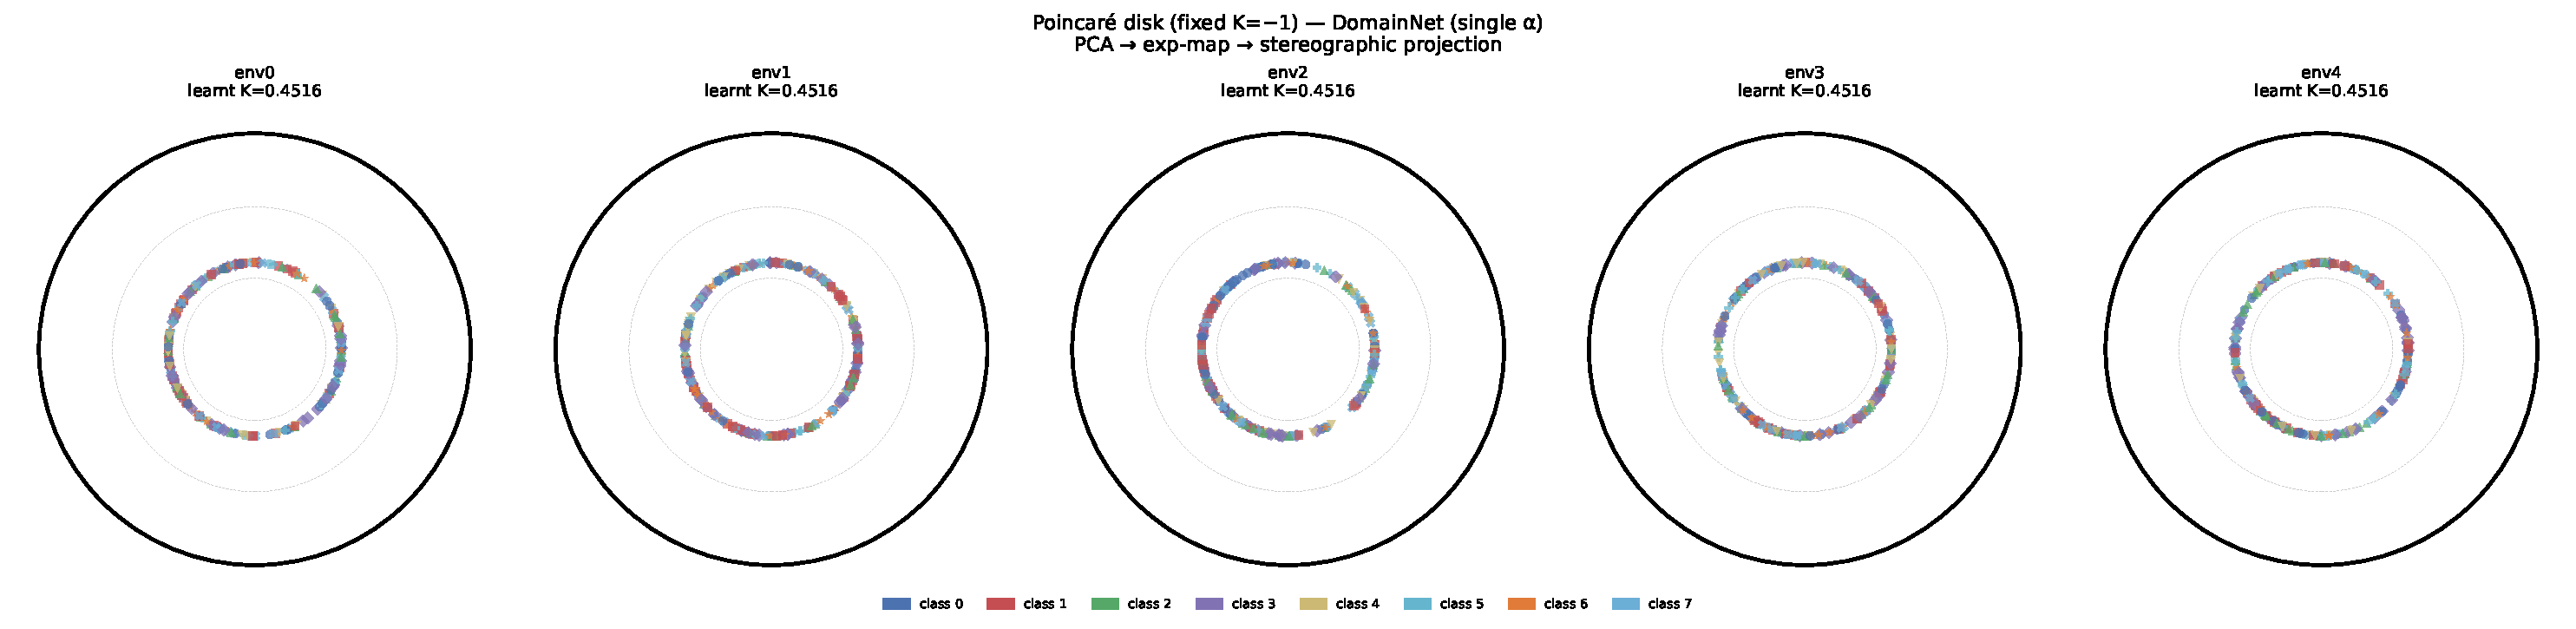
\includegraphics[width=\linewidth]{poincare_hyperdg_domainnet_singlecurv.pdf}
\caption{DomainNet}
\end{subfigure}

\vspace{0.5em}

\begin{subfigure}{0.48\textwidth}
\centering
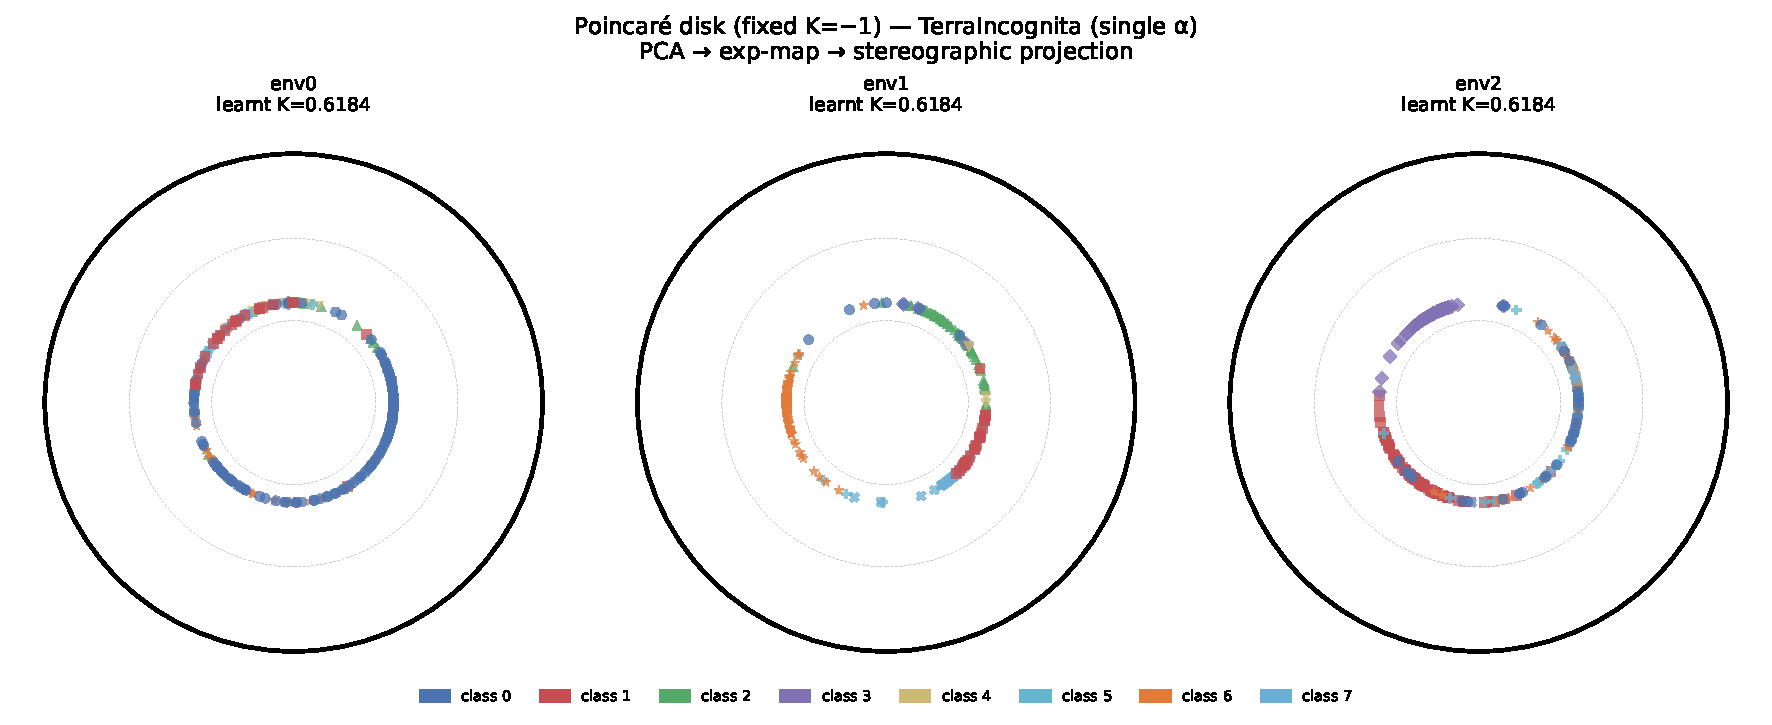
\includegraphics[width=\linewidth]{poincare_hyperdg_terra_singlecurv.pdf}
\caption{TerraIncognita}
\end{subfigure}

\caption{HyperDG using a single shared learnable curvature. Radial distributions become more uniform.}
\end{figure}

%%%%%%%%%%%%%%%%%%%%%%%%%%%%%%%%%%%%%%%%%%%%%%%%%%%%%%%%%%%%%%%%%%%%%%
\subsection{MERU Backbone Visualizations}

\begin{figure}[H]
\centering

\begin{subfigure}{0.48\textwidth}
\centering
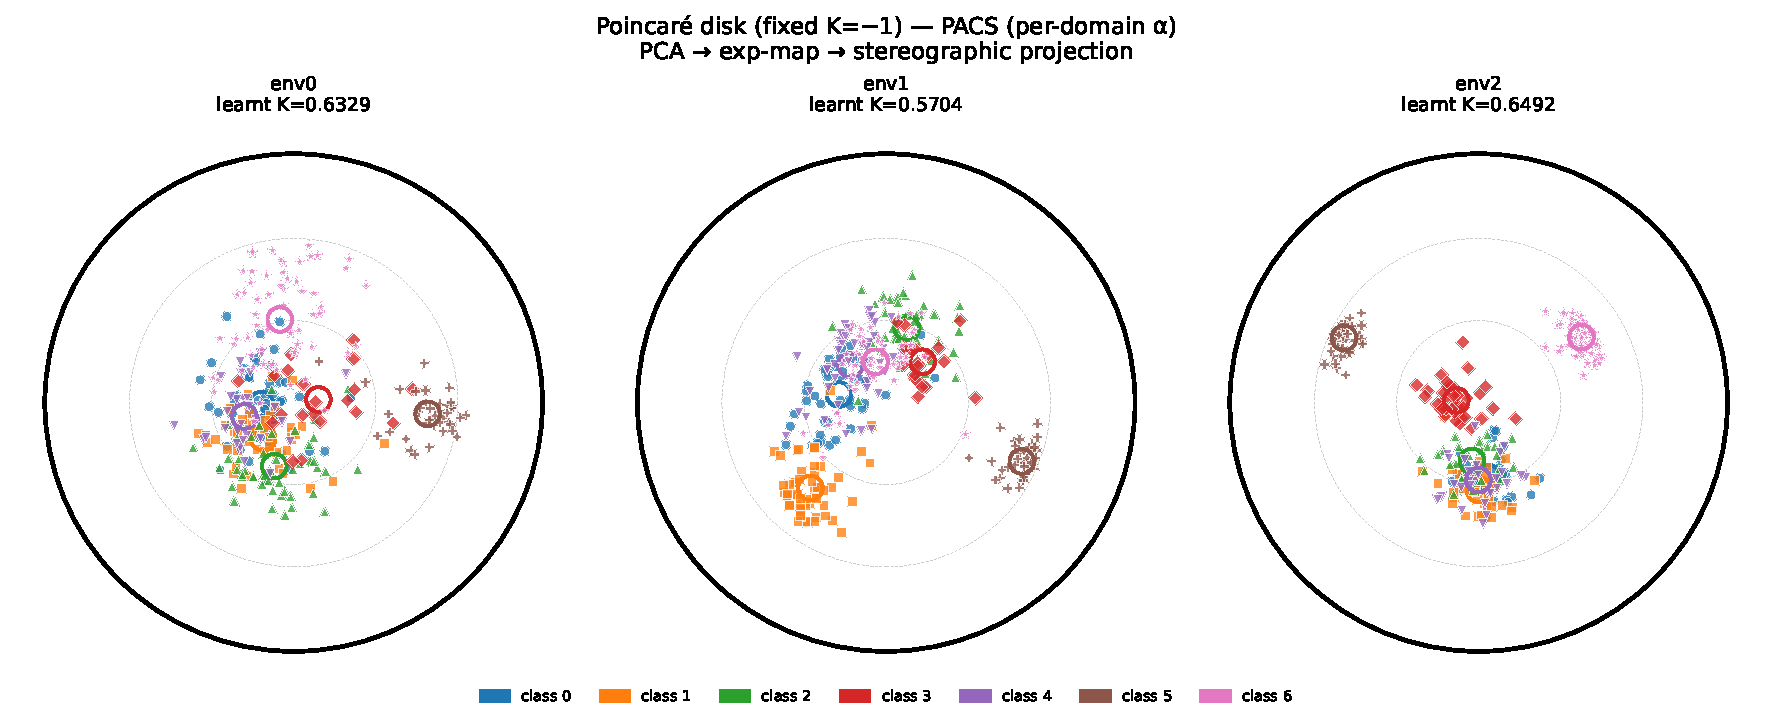
\includegraphics[width=\linewidth]{poincare_meru_pacs_perdomain.pdf}
\caption{PACS + Per-domain}
\end{subfigure}
\hfill
\begin{subfigure}{0.48\textwidth}
\centering
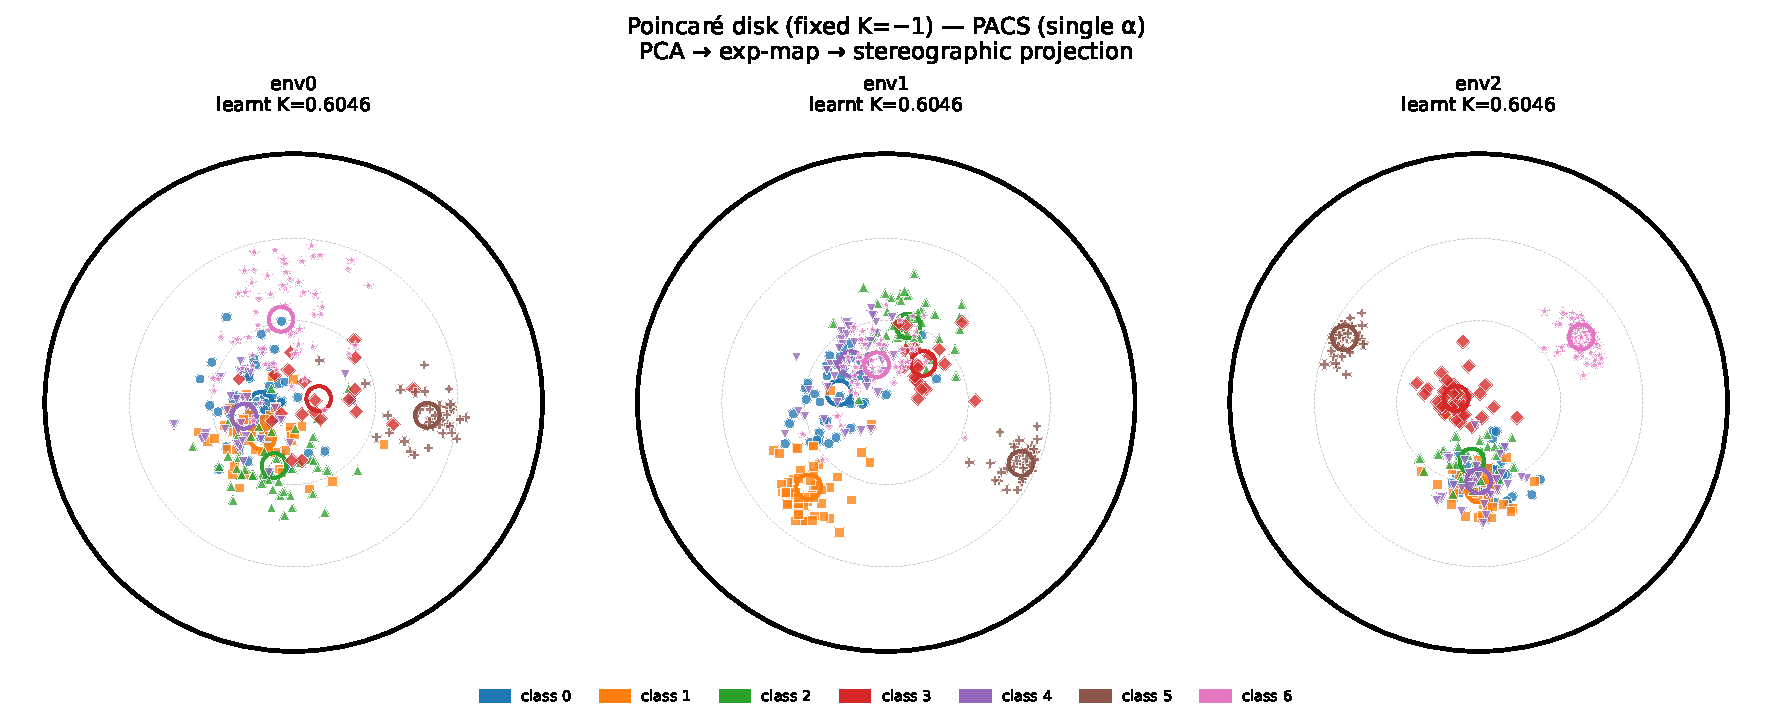
\includegraphics[width=\linewidth]{poincare_meru_pacs_singlecurv.pdf}
\caption{PACS + Single Curvature}
\end{subfigure}

\vspace{0.5em}

\begin{subfigure}{0.48\textwidth}
\centering
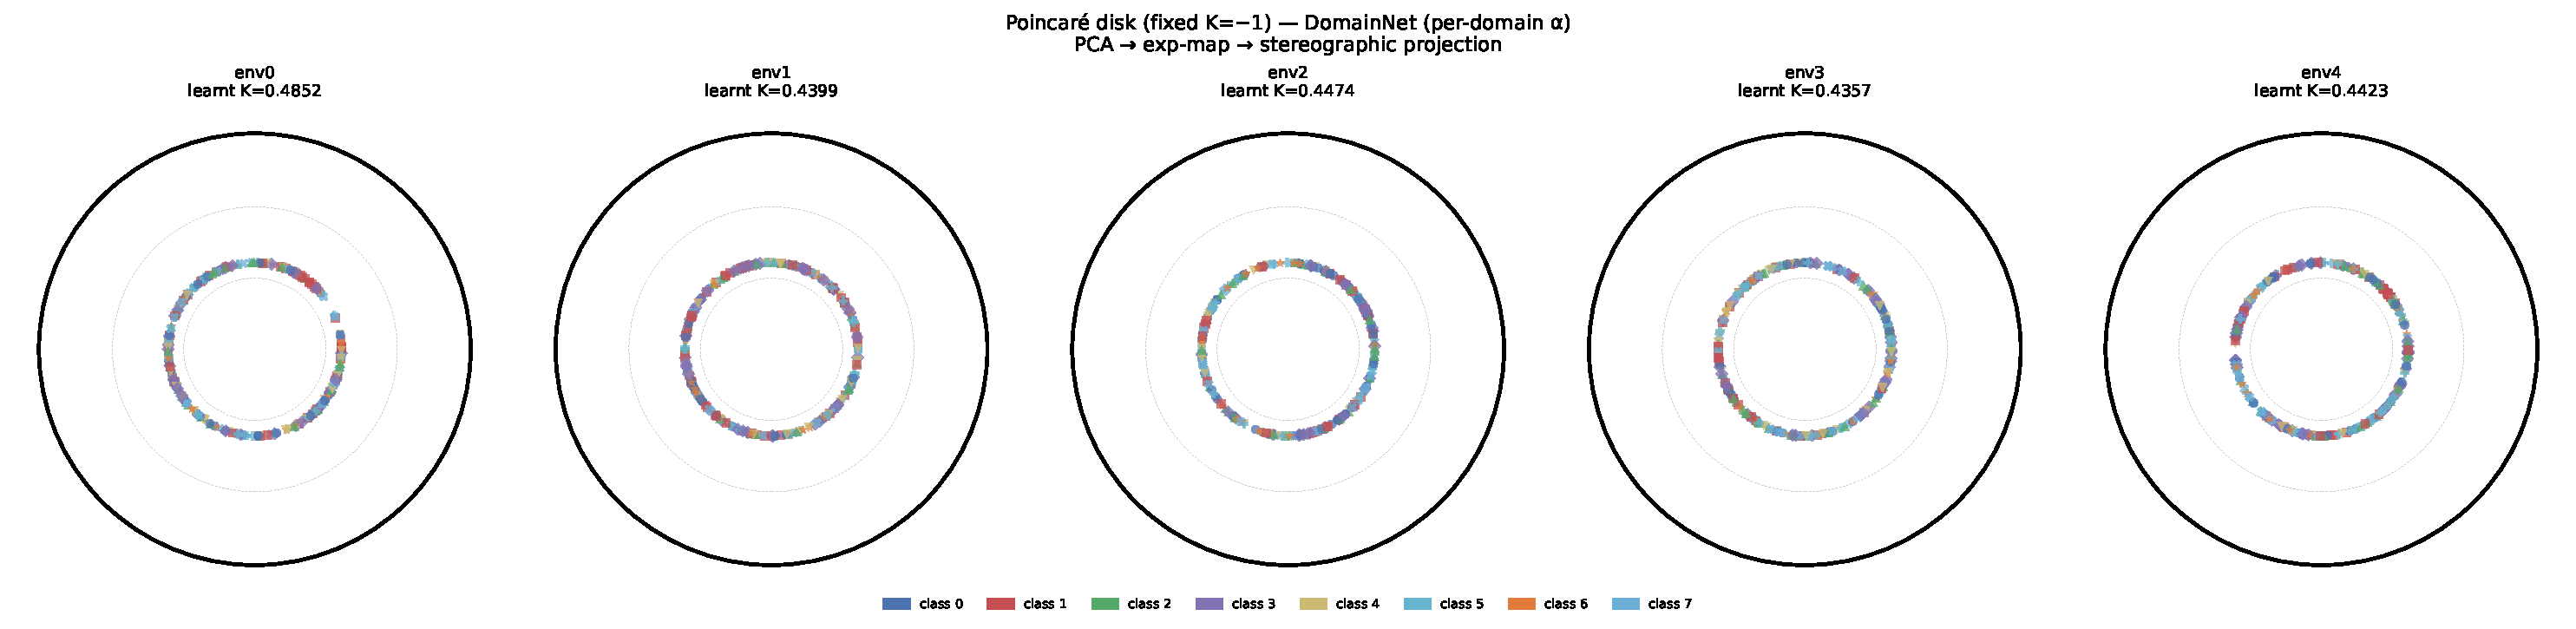
\includegraphics[width=\linewidth]{poincare_meru_domainnet_perdomain.pdf}
\caption{DomainNet + Per-domain}
\end{subfigure}
\hfill
\begin{subfigure}{0.48\textwidth}
\centering
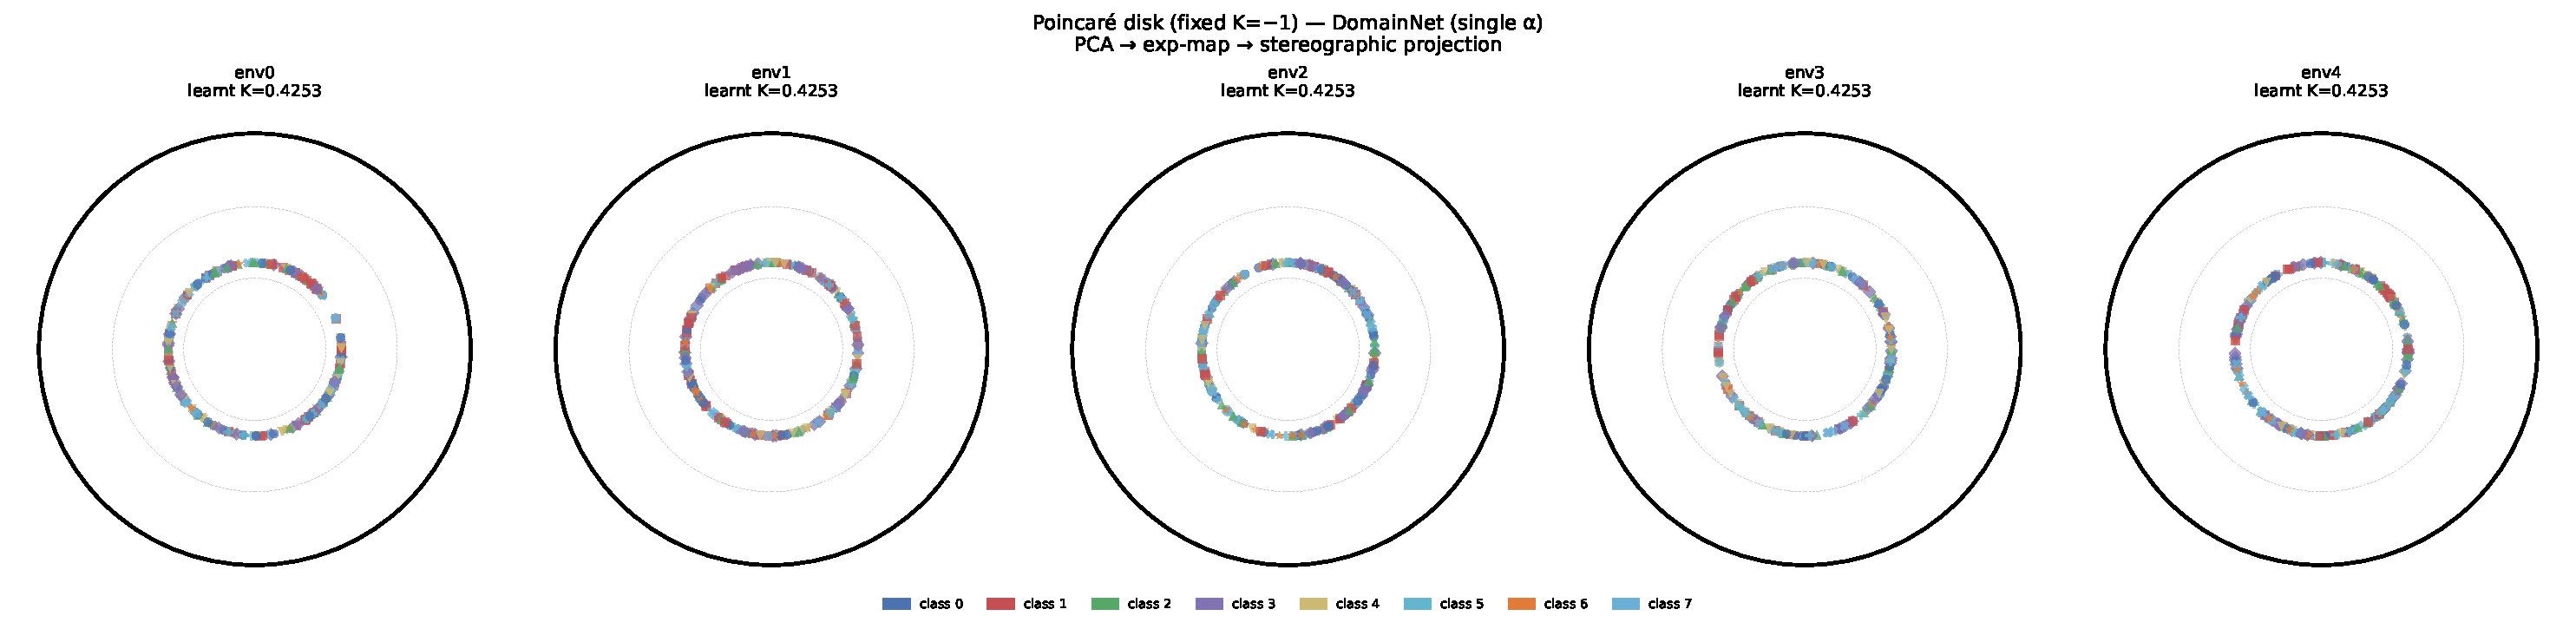
\includegraphics[width=\linewidth]{poincare_meru_domainnet_singlecurv.pdf}
\caption{DomainNet + Single Curvature}
\end{subfigure}

\caption{MERU-based variants exhibit tighter clusters due to stronger hyperbolic priors from pretraining.}
\end{figure}

%%%%%%%%%%%%%%%%%%%%%%%%%%%%%%%%%%%%%%%%%%%%%%%%%%%%%%%%%%%%%%%%%%%%%%
% \section{Curvature Evolution During Training}

% \begin{figure}[H]
% \centering
% \includegraphics[width=0.8\linewidth]{curvature_training_curve.pdf}
% \caption{Evolution of learned curvature parameters during training. Values stabilize rapidly and converge to a narrow band, validating variance regularization.}
% \end{figure}

%%%%%%%%%%%%%%%%%%%%%%%%%%%%%%%%%%%%%%%%%%%%%%%%%%%%%%%%%%%%%%%%%%%%%%
\section{Additional ablation tables}

\subsection{Single shared curvature vs.\ per-domain curvature}

\begin{table}[H]
\centering
\caption{Per-domain learnable $K_i$ vs.\ a single shared learnable $K$
(seed $0$; mean $\pm$ std over the four leave-one-out splits). The two
parameterizations are within ${\pm}0.5$ pp of each other on every
benchmark consistent with the main-paper finding that the per-domain
parameterization is not the source of any geometric benefit. Earlier
draft numbers (PACS $92.2$, VLCS $81.8$, etc.) are superseded by these
reproducible values.}
\begin{tabular}{lccc}
\toprule
Dataset           & Per-domain $K_i$ & Single shared $K$ & $\Delta$ \\
\midrule
PACS              & 84.76 $\pm$ 7.55  & 85.29 $\pm$ 5.23  & $+0.53$ \\
VLCS              & 77.49 $\pm$ 15.38 & 76.21 $\pm$ 16.24 & $-1.28$ \\
OfficeHome        & 66.73 $\pm$ 10.34 & 65.50 $\pm$ 10.11 & $-1.23$ \\
TerraIncognita    & 43.41 $\pm$ 5.45  & 43.25 $\pm$ 3.27  & $-0.16$ \\
DomainNet         & 52.1$^{*}$        & 52.6$^{*}$        & $+0.5$  \\
\bottomrule
\end{tabular}
\\[2pt]
{\footnotesize $^*$ DomainNet rows were not re-evaluated under the new
pipeline (compute-limited) and are shown only for context.}
\end{table}

%%%%%%%%%%%%%%%%%%%%%%%%%%%%%%%%%%%%%%%%%%%%%%%%%%%%%%%%%%%%%%%%%%%%%%
\subsection{Runtime Overhead}

\begin{table}[H]
\centering
\caption{Wall-clock training cost.}
\begin{tabular}{lcc}
\toprule
Method & ms/step & Relative Cost \\
\midrule
ERM & 464.81 & 1.00$\times$ \\
SFT & 581.40 & 1.25$\times$ \\
HyperDG & 458.69 & 0.99$\times$ \\
\bottomrule
\end{tabular}
\end{table}

%%%%%%%%%%%%%%%%%%%%%%%%%%%%%%%%%%%%%%%%%%%%%%%%%%%%%%%%%%%%%%%%%%%%%%
\section{Implementation Notes}

All supplementary experiments use the same optimizer, seeds, splits, and evaluation protocol as the main paper unless otherwise stated.

%%%%%%%%%%%%%%%%%%%%%%%%%%%%%%%%%%%%%%%%%%%%%%%%%%%%%%%%%%%%%%%%%%%%%%
\section{Reproducibility}

All 292 runs (Batches 1--4) are reproducible end-to-end from the released
configurations and aggregation scripts. The repository layout is:
\begin{itemize}[leftmargin=1.5em]
\item \texttt{configs/batch\{1,2,3,4\}/} -- per-batch YAML configurations.
\item \texttt{experiments/batch\{1,2,3,4\}/} -- per-run \texttt{metrics.jsonl} +
      final checkpoints.
\item \texttt{scripts/aggregate\_batch4.py} -- regenerates the multi-seed
      headline table and paired $t$-tests.
\item \texttt{scripts/plot\_curvature\_trajectories.py} -- regenerates the
      trajectory figures and the curvature-spread CSV.
\item \texttt{scripts/plot\_poincare\_disk.py} -- regenerates the
      class-prototype Poincar\'e disks.
\end{itemize}

\section{Acknowledgement of the action editor's feedback}

We thank the action editor for the explicit invitation to embrace the
negative empirical finding and for the strong suggestion that a careful
negative result is a contribution worth publishing. The present revision
attempts to honor that invitation: rather than defending the original
positive claim by tweaking the protocol, we present the controlled
multi-seed comparison, the leave-one-out source-of-gains decomposition,
and the curvature-trajectory diagnostic as the evidence and let the
implications speak for themselves.

\end{document}